\section{Newspaper Pages and CPS-based Condition Setup}
\label{sec:newspaperpages}
%%%%%%%%%%%%%%%%%%%%%%%%%%%%%%%%%%%%%%%%%%%%%%%%%%%%%%%%%%%%%%%%%%%%%%%%%%%%
%%%%%%%%%%%%%%%%%%%%%%%%%%%%%%%%%%%%%%%%%%%%%%%%%%%%%%%%%%%%%%%%%%%%%%%%%%%%

\subsection{Newspaper Pages}
\subsubsection{Original edition}

Each newspaper page combined two components: (1) a \emph{layout file}, defining the geometric arrangement of articles on the page, and (2) a \emph{content file}, providing the textual material for each article (headline, body text, and target font sizes). Because our study focuses on headlines, body text was generated only to fill space within article blocks and was not analyzed.  

In total,  18 newspaper pages were generated, each containing between 8 and 11 articles (see \figref{fig:newspaper-pages}(a)). Below, the construction of layouts, headline sizes, and content are detailed .
\begin{figure}[htbp]
    \centering
    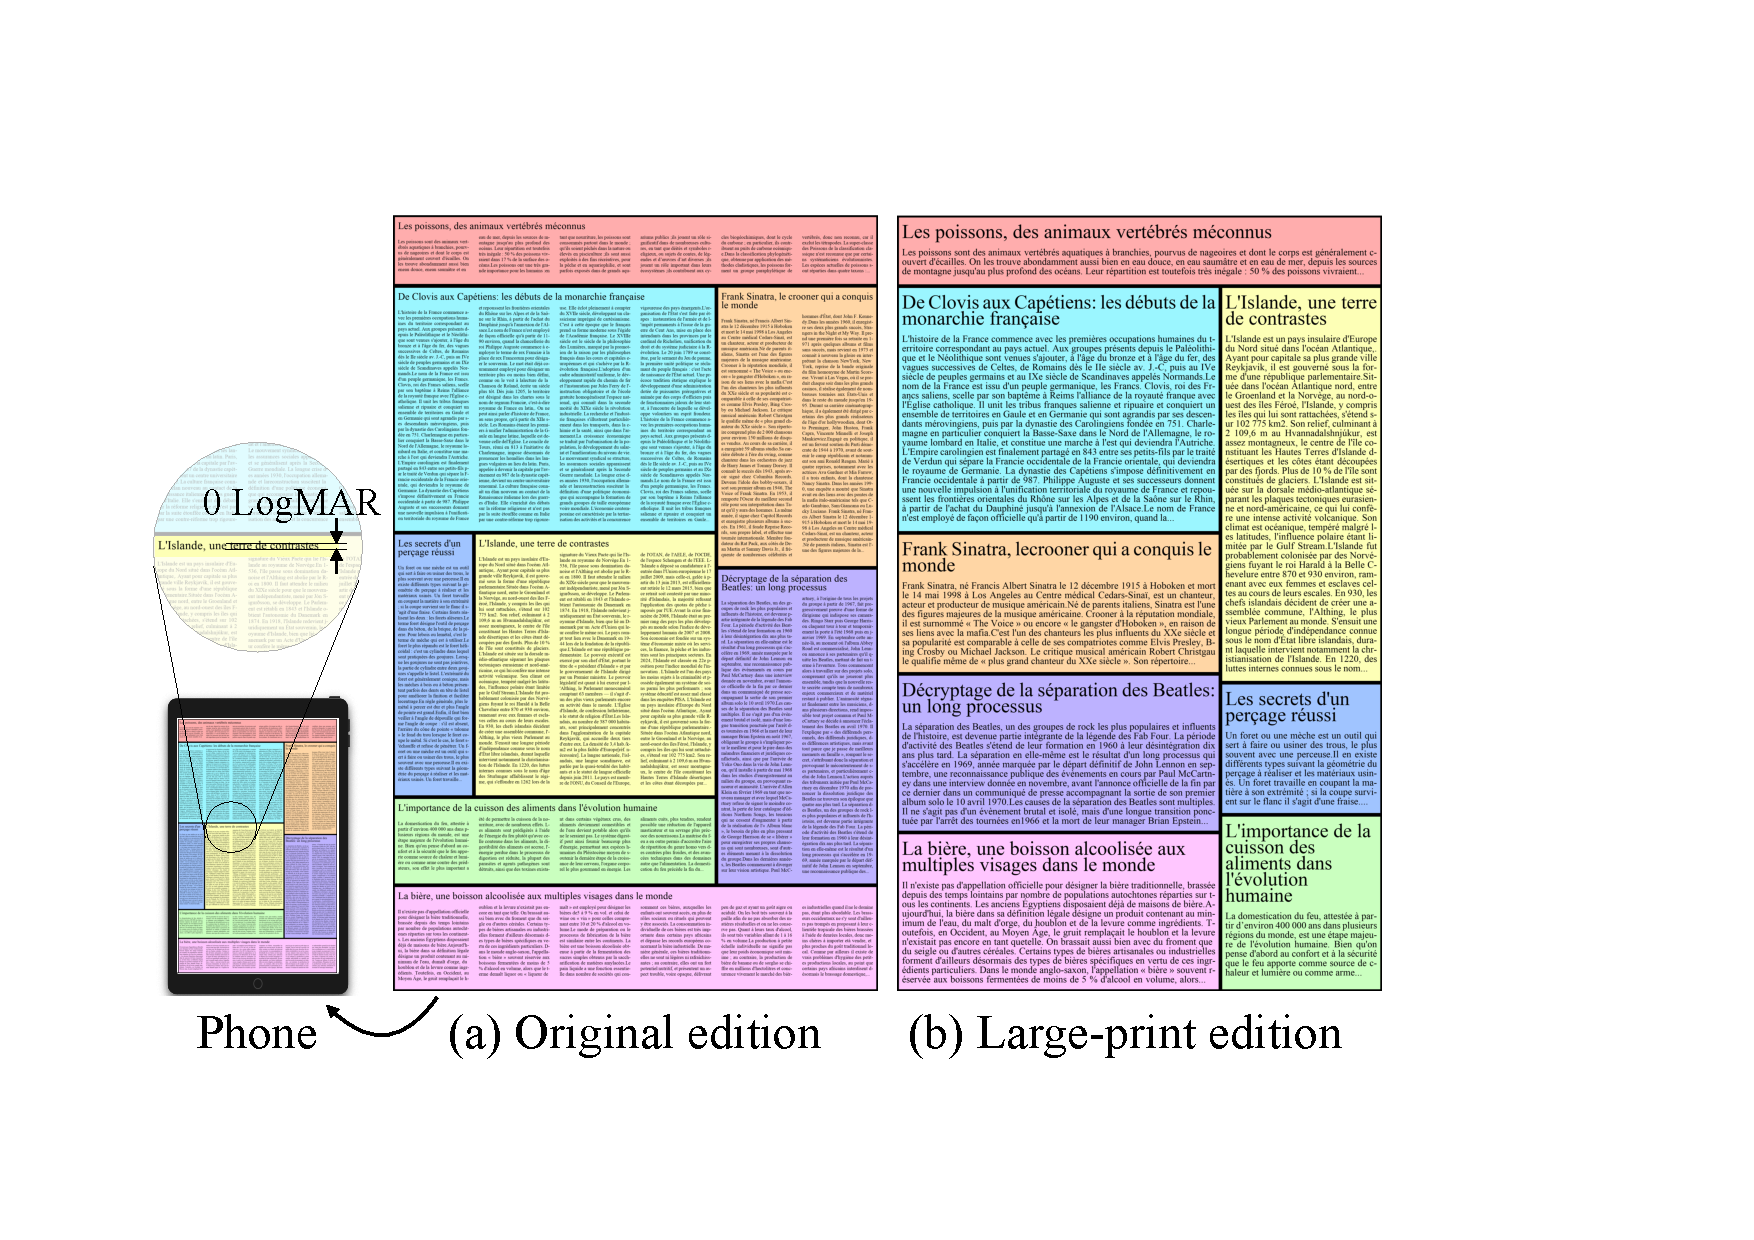
\includegraphics[width=\widthForOneImage]{img/newspaper-material.pdf}
    \caption{
    Examples of newspaper pages: (a) original edition used in condition \condonenot, and (b) corresponding large-print edition used in condition \condtwonot,  with a $\times 2$ magnification.  
    Colors indicate matching articles across the two versions (i.e., occupying the same area on the page). The textual content differs between (a) and (b) to avoid repetition effects, but was balanced in headline length. The left-hand side illustrate how the original edition would look in a phone, which is the display used to define the headline size in LogMAR.}

    \label{fig:newspaper-pages}
\end{figure}

\paragraph{Font size.}  
Headline size was fixed to correspond to a visual angle of $0$ logMAR when displayed on the phone at a viewing distance of 40\,cm (\figref{fig:newspaper-pages}(a); see \secref{sec:condition-definition}). This $0$ logMAR size was intentionally chosen to challenge normally-sighted participants, as it requires zooming for comfortable reading~\cite{calabrese_baseline_2016}. Body text size was set heuristically to half the headline size. 
%Details on converting logMAR values to pixel dimensions are provided in Appendix~\ref{sec:appendix-font-size}.

\paragraph{Layouts.}  
Layouts were created manually from annotated front pages of the \NYT. Nine layout files were produced ($\layoutset=\{l_i\}_{i=1,..,9}$), each specifying the number of articles, their position, and their dimensions (width and height in mm). Based on these dimensions and the font size,  the required article length in characters and lines are extrapolated. 

More precisely, concerning headlines, to match the New York Times design, headline lengths were analyzed, relative to article width (number of columns). This showed that headlines in narrower articles (spanning fewer than two columns) typically used up to three lines, while those in wider articles (three or more columns) almost always fit on a single line. The objective is to replicate this distribution when generating the stimuli headlines (see example in \figref{fig:newspaper-pages}(a)). 

\paragraph{Content.}  
Given article length specifications, three distinct content files for each layout file were created, yielding a total of 27 sets of article content $\contentset=\{c_{ij}\}_{i=1...9, j=1,2,3}$. This ensured that participants were not exposed to the same material across conditions (\condzeronot, \condonenot, \condtwonot), avoiding memory bias. Content files were created in R~\cite{R} by selecting the article's text from the web. For each article, a matching headline was then generated automatically with MistralAI~\cite{mistralai}. This LLM-based approach was utilized to generate controlled media stimuli with uniform linguistic difficulty. This ensured that the behavioral integrity of the reading paths was measured against standardized content, eliminating potential engagement biases or emotional confounding that could arise from prior knowledge of real-world news events.

As a starter, a list of 364 key words (e.g., dog, Paris, etc.) was manually written to serve as article topics and sorted within 30 general themes (e.g., animals, cities, etc.). For each keyword, the R~\cite{R} \emph{getwiki} library was used to search the web and extract the first paragraph of the top 20 Wikipedia and Vikidia pages (in French) matching the search result. This resulted in a list of 11,565 articles. Using a custom-based routine in R, this list was searched to assign the optimal candidate articles to each layout file, based on the required character length, checking that the same theme was only chosen once within a single page to avoid redundant topics. 

Last, MistralAI was prompted from R to generate a list of 10 titles per article automatically. The prompt sent to MistralAI was as follows: "Create 10 possible headlines in the style of a journal article, in French, with approximately \emph{n} characters (space included), about the following article \emph{t}", \emph{n} being the number of characters given by the layout files and \emph{t} being the text of the article. Each output was manually inspected to obtain the optimal headline. 

\subsubsection{Large-print edition}

For each original edition,  a large-print counterpart was by applying the automatic re-layouting method from Gallardo et al.~\cite{gallardo}. This approach corresponds to a simplified single-objective version of the method presented in Chapter~\ref{chapter:pagegen}, specifically designed to generate large-print layouts for newspapers. It addresses the limitations of simple font scaling (which can cause text overflows and break entry points because original layouts were not designed for increased sizes~\cite{gallardo}). This method takes an original edition and a font size magnification factor to apply, and uses an evolutionary algorithm to reorganize layouts in a way that optimizes the number of lines of each headline and the aesthetic quality of the layout e.g., alignment of articles, visual balance, etc. It is crucial to note that the goal of this adaptation is structural integrity over the preservation of absolute coordinates. While the articles are re-positioned to accommodate the larger font size, the 2D layout topology is maintained.

In particular, this method is fed with a layout $l_i$ and one content set ($c_{i,1}$), together with a magnification factor of $\times 2$, which comfortably covers the critical print size spectrum across both participant groups (see \secref{sec:condition-definition}).  Only $c_{i,1}$ was used for generating these layouts (since $c_{i,2}$ and $c_{i,3}$ are equivalent in terms of length). The output is a new large-print layout $\largeprintset=\{l'_i\}_{i=1,...,9}$ (\figref{fig:newspaper-pages}(b)). The large-print edition was obtained by combining the large-print layout with one of the three equivalent content files for that page. Note that in the large-print edition, a larger font size inevitably prevents the full body text of each article from being displayed in the overview. This is an inherent feature of these large-print digital editions, which, like existing kiosk-style news applications, are designed primarily to support scanning and discovery of articles. Readers would use the overview to identify entry points (e.g., headlines), and then would access the full content in a dedicated single-page reading mode.


\subsection{Conditions setup based on CPS}
\label{sec:condition-definition}
%%%%%%%%%%%%%%%%%%%%%%%%%%%%%%%%%%%%%%%%%%%%%%%%%%%%%%%%%%%%%%%%%%%%%%%%%%%%
%%%%%%%%%%%%%%%%%%%%%%%%%%%%%%%%%%%%%%%%%%%%%%%%%%%%%%%%%%%%%%%%%%%%%%%%%%%%

To recap, the goal is to design an experiment where condition \condonenot forces participants to use gesture-based magnification, as the original edition’s headlines are deliberately too small to read comfortably, while condition \condtwonot allows participants to read the large-print edition without any magnification. Importantly, for each participant, both conditions are presented on the same device and at the same head-to-screen distance. The procedure to achieve this setup is detailed in the following steps.

\subsubsection{Estimation of the CPS}

To assess participants’ CPS,  a standardized reading test based on the MNREAD chart was applied~\cite{legge1992psychophysics,mansfield1993}. The MNREAD is a continuous-text reading acuity chart consisting of short sentences presented at progressively smaller print sizes. Reading speed is plotted as a function of print size, producing the characteristic MNREAD curve: a plateau of constant reading speed at larger sizes, followed by a sharp decline once print falls below a critical threshold. The CPS is defined as the smallest print size that still supports maximum reading speed, i.e., the lower bound of the plateau~\cite{legge2006}.

\subsubsection{Headline size in LogMAR}

The visual angle of headlines depends on two factors: the device’s screen size and the viewing distance. Given a participant’s CPS, the goal is therefore to select the appropriate device and distance so that the headline size of the original edition in \condonenot is smaller than the CPS, while the headline size of the large-print edition in \condtwonot is larger than the CPS. When multiple configurations are possible, we systematically choose the one that yields headline sizes closest to the CPS. This principle is illustrated in \figref{fig:conditions-setup}(a).
\begin{figure}[htbp]
    \centering
    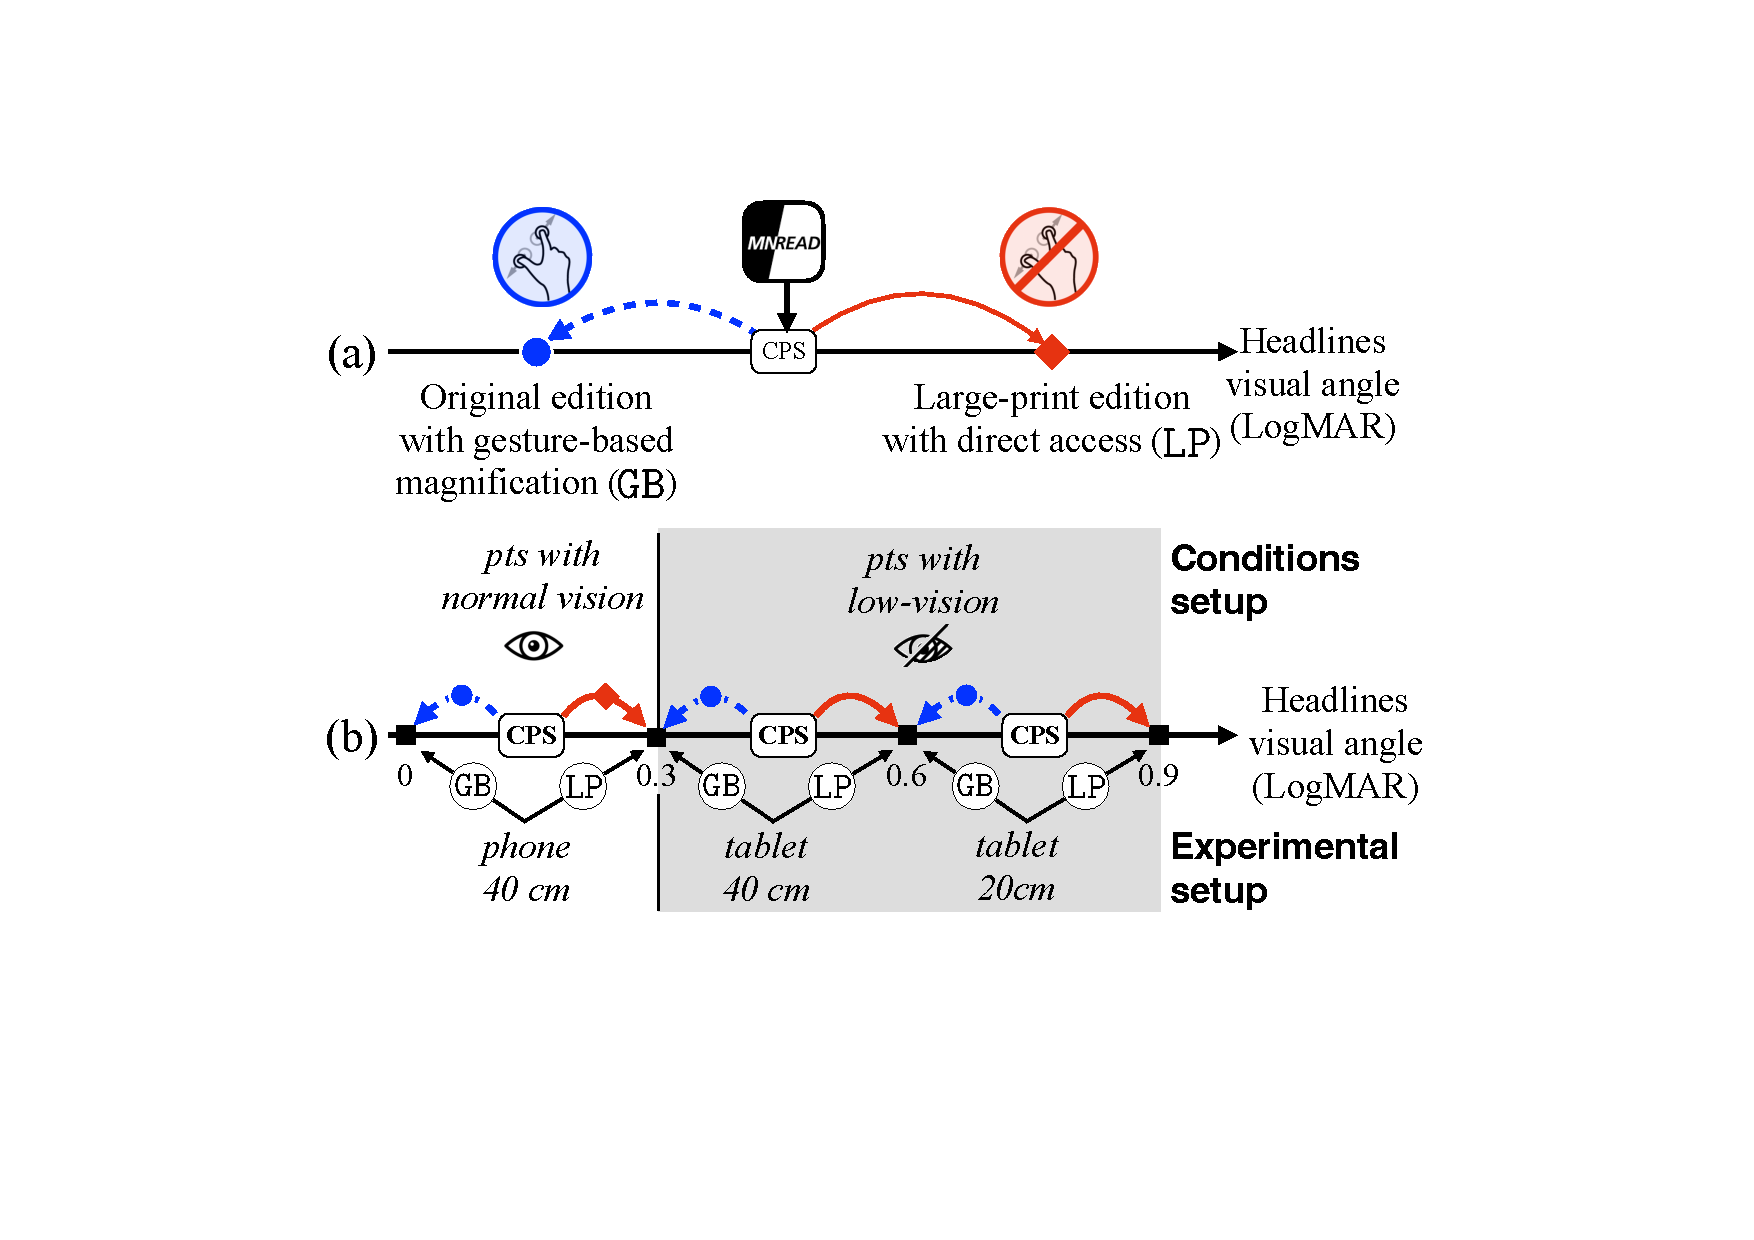
\includegraphics[width=\widthForOneImage]{img/conditions-setup.pdf}
    \caption{
    Experimental condition setup based on CPS.  
    (a) General principle: headline visual angles in both conditions are selected around the participant’s CPS value obtained from an MNREAD test.  
    (b) Device and viewing distance configuration depending on the scenario: for participants \NV ($0 \leq CPS \leq 0.3$), the experiment was conducted on a phone at a fixed distance of 40\,cm; for participants \LV ($0.3 \leq CPS \leq 0.9$), the experiment was conducted on a tablet, with the viewing distance adjusted according to the CPS value.}
    \label{fig:conditions-setup}
\end{figure}

A custom-designed app, developed using React Native framework, was deployed for the application of this protocol.
Regarding this, we use two different Android devices:
\begin{itemize}
    \item \textbf{Phone:} Google Pixel~7, featuring a 7.3-inch screen with a maximum resolution of $1080 \times 2400$ pixels.  
    \item \textbf{Tablet:} Samsung Galaxy Tab S9 FE+, featuring a 12.4-inch screen with a maximum resolution of $1600 \times 2560$ pixels.  
\end{itemize}

These specifications, combined with adjustments of the viewing distance, allow to cover participants with CPS values ranging from 0 to 0.9. The actual configuration depended on each participant’s CPS, as illustrated in \figref{fig:conditions-setup}(b). For participants \NV,  the specified phone was set at a fixed viewing distance of 40\,cm. For participants \LV, the tablet was used instead, with the viewing distance adjusted according to their CPS.
